\begin{figure}
  \begin{center}
    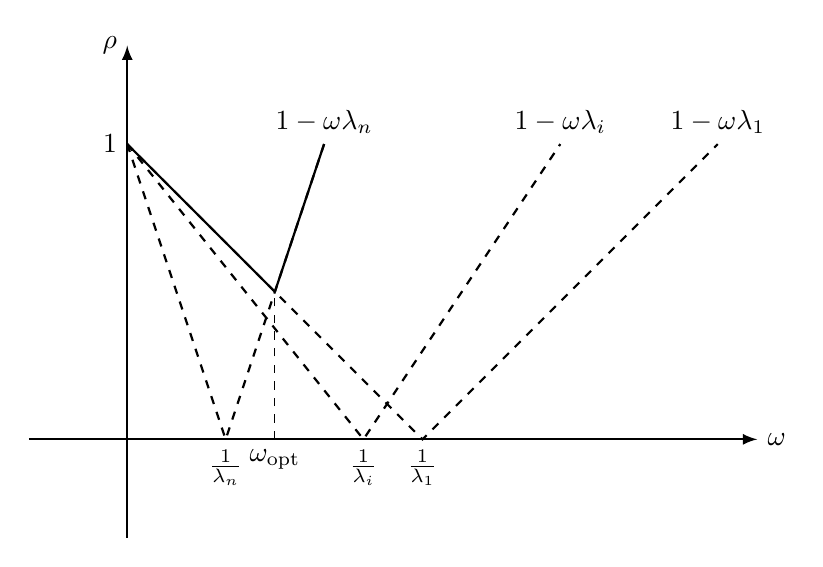
\begin{tikzpicture}[scale=2.5,>=latex]
      \coordinate (o) at (0,0);
      \coordinate (x) at (1,1);
      \coordinate (x1) at (-0.5,0);
      \coordinate (x2) at (3.2,0);
      \coordinate (y1) at (0,-0.5);
      \coordinate (y2) at (0,2);
      %
      % Axes:
      \draw [->,thick] (x1)--(x2) node (xaxis) [right] {$\omega$};
      \draw [->,thick] (y1)--(y2) node (yaxis) [left] {$\rho$};
      \draw [black, dashed] (0.75,0) node[below] {$\omega_{\rm opt}$}--(0.75, 0.75);
      \draw [thick] (0,1.5) node (xaxis) [left] {1}--(0.75,0.75);
      \draw [thick, dashed,black](0,1.5)--(1.5,0)node[below] {$\frac{1}{\lambda_1}$} --(3,1.5) node[above] {$\abs{1-\omega\lambda_1}$};
      \draw [thick, dashed,black](0,1.5)--(1.2,0)node[below] {$\frac{1}{\lambda_i}$} --(2.2,1.5) node[above] {$\abs{1-\omega\lambda_i}$};
      \draw [thick, dashed,black](0,1.5)--(0.5,0) node[below] {$\frac{1}{\lambda_n}$}--(1.0,1.5);
      \draw [thick] (0.75,0.75)--(1.0,1.5) node[above] {$\abs{1-\omega\lambda_n}$};
    \end{tikzpicture}
  \end{center}
  \caption{The curve $\rho(\msfT_{{\rm R}})$ (in solid black) as a function of $\omega$.}
\label{fig:optomega}
\end{figure}
